\chapter{Introduction}

\eWoms aims to be a generic framework for the simulation of multiphase
fluid flow and transport processes in porous media using continuum
mechanical approaches.  At the same time, \eWoms aims to deliver
top-notch computational performance, high flexibility, a sound
software architecture and the ability to run on anything from single
processor systems to highly parallel supercomputers with specialized
hardware architectures.

The means to achieve these somewhat contradictory goals are the
thorough use of object oriented design in conjunction with template
programming. These requirements motivated the decision to use
\Cplusplus as the implementation language for \eWoms.

One of the more complex issues when dealing with parallel continuum
models is managing the grids used for the spatial discretization of
the physical model. To date, no generic and efficient approach exists
for all possible cases, so \eWoms is build on top of \Dune, the
\textbf{D}istributed and \textbf{U}nified \textbf{N}umerics
\textbf{E}nvironment~\cite{DUNE-HP}. \Dune provides a generic interface
to many existing grid management libraries such as UG~\cite{UG-HP},
ALBERTA~\cite{ALBERTA-HP}, ALUGrid~\cite{ALUGRID-HP} and a few
more. DUNE also extensively uses template programming in order to
achieve minimal overhead when accessing the underlying grid
libraries\footnote{In fact, the performance penalty resulting from the
use of \Dune's grid interface is usually negligible~\cite{BURRI2006}.}.
\begin{figure}[hbt]
  \centering 
  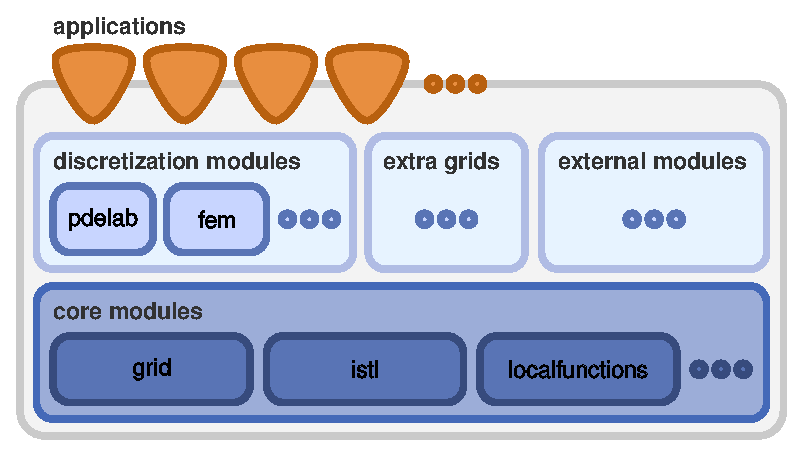
\includegraphics[width=.5\linewidth, keepaspectratio]{EPS/dunedesign}
  \caption{
    \label{fig:dune-design}
    A high-level overview of \Dune's design is available on the project's
    web site~\cite{DUNE-HP}.
  }
\end{figure}

DUNE's grid interface is independent of the spatial dimension of the
underlying grid. For this purpose, it uses the concept of
co-dimensional entities. Roughly speaking, an entity of co-dimension
$0$ constitutes a cell, co-dimension $1$ entities are faces between
cells, co-dimension $1$ are edges, and so on until co-dimension $n$
which are the cell's vertices.  The \Dune grid interface generally
assumes that all entities are convex polytopes, which means that it
must be possible to express each entity as the convex hull of a set of
vertices. For the sake of efficiency, all entities are further expressed in terms
of so-called reference elements which are transformed to the actual
spatial incarnation within the grid by a so-called geometry
function. Here, a reference element for an
entity can be thought of as a prototype for the actual grid
entity. For example, if we used a grid which applied hexahedrons as cells,
the reference element for each cell would be the unit cube $[0, 1]^3$
and the geometry function would scale and translate the cube so that
it matches the grid's cell. For a more thorough description of \Dune's
grid definition, see~\cite{BASTIAN2008}.

In addition to the grid interface, \Dune also provides quite a few
additional modules, of which the \texttt{dune-localfunctions} and
\texttt{dune-istl} modules are the most relevant in the context of
this handbook. \texttt{dune-localfunctions} provides a set of generic
finite element shape functions, while \texttt{dune-istl} is the
\textbf{I}terative \textbf{S}olver \textbf{T}emplate \textbf{L}ibrary
and provides generic, highly optimized linear algebra routines for
solving the generated systems.

\eWoms comes in form of an additional module \Dune module
'\texttt{ewoms}'.  It depends on the \Dune core modules
\texttt{dune-common}, \texttt{dune-grid}, \texttt{dune-istl}, and on
\texttt{dune-localfunctions}.  The main intention of \eWoms is to
provide a framework for an easy and efficient implementation of new
physical models for porous media flow problems, ranging from problem
formulation and the selection of spatial and temporal discretization
schemes as well as nonlinear solvers, to general concepts for model
coupling.  Moreover, \eWoms includes ready-to-use numerical models and
a few example applications.

%%% Local Variables: 
%%% mode: latex
%%% TeX-master: "ewoms-handbook"
%%% End: 
